
% Default to the notebook output style

    


% Inherit from the specified cell style.




    
\documentclass[11pt]{article}

    
    
    \usepackage[T1]{fontenc}
    % Nicer default font (+ math font) than Computer Modern for most use cases
    \usepackage{mathpazo}

    % Basic figure setup, for now with no caption control since it's done
    % automatically by Pandoc (which extracts ![](path) syntax from Markdown).
    \usepackage{graphicx}
    % We will generate all images so they have a width \maxwidth. This means
    % that they will get their normal width if they fit onto the page, but
    % are scaled down if they would overflow the margins.
    \makeatletter
    \def\maxwidth{\ifdim\Gin@nat@width>\linewidth\linewidth
    \else\Gin@nat@width\fi}
    \makeatother
    \let\Oldincludegraphics\includegraphics
    % Set max figure width to be 80% of text width, for now hardcoded.
    \renewcommand{\includegraphics}[1]{\Oldincludegraphics[width=.8\maxwidth]{#1}}
    % Ensure that by default, figures have no caption (until we provide a
    % proper Figure object with a Caption API and a way to capture that
    % in the conversion process - todo).
    \usepackage{caption}
    \DeclareCaptionLabelFormat{nolabel}{}
    \captionsetup{labelformat=nolabel}

    \usepackage{adjustbox} % Used to constrain images to a maximum size 
    \usepackage{xcolor} % Allow colors to be defined
    \usepackage{enumerate} % Needed for markdown enumerations to work
    \usepackage{geometry} % Used to adjust the document margins
    \usepackage{amsmath} % Equations
    \usepackage{amssymb} % Equations
    \usepackage{textcomp} % defines textquotesingle
    % Hack from http://tex.stackexchange.com/a/47451/13684:
    \AtBeginDocument{%
        \def\PYZsq{\textquotesingle}% Upright quotes in Pygmentized code
    }
    \usepackage{upquote} % Upright quotes for verbatim code
    \usepackage{eurosym} % defines \euro
    \usepackage[mathletters]{ucs} % Extended unicode (utf-8) support
    \usepackage[utf8x]{inputenc} % Allow utf-8 characters in the tex document
    \usepackage{fancyvrb} % verbatim replacement that allows latex
    \usepackage{grffile} % extends the file name processing of package graphics 
                         % to support a larger range 
    % The hyperref package gives us a pdf with properly built
    % internal navigation ('pdf bookmarks' for the table of contents,
    % internal cross-reference links, web links for URLs, etc.)
    \usepackage{hyperref}
    \usepackage{longtable} % longtable support required by pandoc >1.10
    \usepackage{booktabs}  % table support for pandoc > 1.12.2
    \usepackage[inline]{enumitem} % IRkernel/repr support (it uses the enumerate* environment)
    \usepackage[normalem]{ulem} % ulem is needed to support strikethroughs (\sout)
                                % normalem makes italics be italics, not underlines
    

    
    
    % Colors for the hyperref package
    \definecolor{urlcolor}{rgb}{0,.145,.698}
    \definecolor{linkcolor}{rgb}{.71,0.21,0.01}
    \definecolor{citecolor}{rgb}{.12,.54,.11}

    % ANSI colors
    \definecolor{ansi-black}{HTML}{3E424D}
    \definecolor{ansi-black-intense}{HTML}{282C36}
    \definecolor{ansi-red}{HTML}{E75C58}
    \definecolor{ansi-red-intense}{HTML}{B22B31}
    \definecolor{ansi-green}{HTML}{00A250}
    \definecolor{ansi-green-intense}{HTML}{007427}
    \definecolor{ansi-yellow}{HTML}{DDB62B}
    \definecolor{ansi-yellow-intense}{HTML}{B27D12}
    \definecolor{ansi-blue}{HTML}{208FFB}
    \definecolor{ansi-blue-intense}{HTML}{0065CA}
    \definecolor{ansi-magenta}{HTML}{D160C4}
    \definecolor{ansi-magenta-intense}{HTML}{A03196}
    \definecolor{ansi-cyan}{HTML}{60C6C8}
    \definecolor{ansi-cyan-intense}{HTML}{258F8F}
    \definecolor{ansi-white}{HTML}{C5C1B4}
    \definecolor{ansi-white-intense}{HTML}{A1A6B2}

    % commands and environments needed by pandoc snippets
    % extracted from the output of `pandoc -s`
    \providecommand{\tightlist}{%
      \setlength{\itemsep}{0pt}\setlength{\parskip}{0pt}}
    \DefineVerbatimEnvironment{Highlighting}{Verbatim}{commandchars=\\\{\}}
    % Add ',fontsize=\small' for more characters per line
    \newenvironment{Shaded}{}{}
    \newcommand{\KeywordTok}[1]{\textcolor[rgb]{0.00,0.44,0.13}{\textbf{{#1}}}}
    \newcommand{\DataTypeTok}[1]{\textcolor[rgb]{0.56,0.13,0.00}{{#1}}}
    \newcommand{\DecValTok}[1]{\textcolor[rgb]{0.25,0.63,0.44}{{#1}}}
    \newcommand{\BaseNTok}[1]{\textcolor[rgb]{0.25,0.63,0.44}{{#1}}}
    \newcommand{\FloatTok}[1]{\textcolor[rgb]{0.25,0.63,0.44}{{#1}}}
    \newcommand{\CharTok}[1]{\textcolor[rgb]{0.25,0.44,0.63}{{#1}}}
    \newcommand{\StringTok}[1]{\textcolor[rgb]{0.25,0.44,0.63}{{#1}}}
    \newcommand{\CommentTok}[1]{\textcolor[rgb]{0.38,0.63,0.69}{\textit{{#1}}}}
    \newcommand{\OtherTok}[1]{\textcolor[rgb]{0.00,0.44,0.13}{{#1}}}
    \newcommand{\AlertTok}[1]{\textcolor[rgb]{1.00,0.00,0.00}{\textbf{{#1}}}}
    \newcommand{\FunctionTok}[1]{\textcolor[rgb]{0.02,0.16,0.49}{{#1}}}
    \newcommand{\RegionMarkerTok}[1]{{#1}}
    \newcommand{\ErrorTok}[1]{\textcolor[rgb]{1.00,0.00,0.00}{\textbf{{#1}}}}
    \newcommand{\NormalTok}[1]{{#1}}
    
    % Additional commands for more recent versions of Pandoc
    \newcommand{\ConstantTok}[1]{\textcolor[rgb]{0.53,0.00,0.00}{{#1}}}
    \newcommand{\SpecialCharTok}[1]{\textcolor[rgb]{0.25,0.44,0.63}{{#1}}}
    \newcommand{\VerbatimStringTok}[1]{\textcolor[rgb]{0.25,0.44,0.63}{{#1}}}
    \newcommand{\SpecialStringTok}[1]{\textcolor[rgb]{0.73,0.40,0.53}{{#1}}}
    \newcommand{\ImportTok}[1]{{#1}}
    \newcommand{\DocumentationTok}[1]{\textcolor[rgb]{0.73,0.13,0.13}{\textit{{#1}}}}
    \newcommand{\AnnotationTok}[1]{\textcolor[rgb]{0.38,0.63,0.69}{\textbf{\textit{{#1}}}}}
    \newcommand{\CommentVarTok}[1]{\textcolor[rgb]{0.38,0.63,0.69}{\textbf{\textit{{#1}}}}}
    \newcommand{\VariableTok}[1]{\textcolor[rgb]{0.10,0.09,0.49}{{#1}}}
    \newcommand{\ControlFlowTok}[1]{\textcolor[rgb]{0.00,0.44,0.13}{\textbf{{#1}}}}
    \newcommand{\OperatorTok}[1]{\textcolor[rgb]{0.40,0.40,0.40}{{#1}}}
    \newcommand{\BuiltInTok}[1]{{#1}}
    \newcommand{\ExtensionTok}[1]{{#1}}
    \newcommand{\PreprocessorTok}[1]{\textcolor[rgb]{0.74,0.48,0.00}{{#1}}}
    \newcommand{\AttributeTok}[1]{\textcolor[rgb]{0.49,0.56,0.16}{{#1}}}
    \newcommand{\InformationTok}[1]{\textcolor[rgb]{0.38,0.63,0.69}{\textbf{\textit{{#1}}}}}
    \newcommand{\WarningTok}[1]{\textcolor[rgb]{0.38,0.63,0.69}{\textbf{\textit{{#1}}}}}
    
    
    % Define a nice break command that doesn't care if a line doesn't already
    % exist.
    \def\br{\hspace*{\fill} \\* }
    % Math Jax compatability definitions
    \def\gt{>}
    \def\lt{<}
    % Document parameters
    \title{Bookings}
    
    
    

    % Pygments definitions
    
\makeatletter
\def\PY@reset{\let\PY@it=\relax \let\PY@bf=\relax%
    \let\PY@ul=\relax \let\PY@tc=\relax%
    \let\PY@bc=\relax \let\PY@ff=\relax}
\def\PY@tok#1{\csname PY@tok@#1\endcsname}
\def\PY@toks#1+{\ifx\relax#1\empty\else%
    \PY@tok{#1}\expandafter\PY@toks\fi}
\def\PY@do#1{\PY@bc{\PY@tc{\PY@ul{%
    \PY@it{\PY@bf{\PY@ff{#1}}}}}}}
\def\PY#1#2{\PY@reset\PY@toks#1+\relax+\PY@do{#2}}

\expandafter\def\csname PY@tok@w\endcsname{\def\PY@tc##1{\textcolor[rgb]{0.73,0.73,0.73}{##1}}}
\expandafter\def\csname PY@tok@c\endcsname{\let\PY@it=\textit\def\PY@tc##1{\textcolor[rgb]{0.25,0.50,0.50}{##1}}}
\expandafter\def\csname PY@tok@cp\endcsname{\def\PY@tc##1{\textcolor[rgb]{0.74,0.48,0.00}{##1}}}
\expandafter\def\csname PY@tok@k\endcsname{\let\PY@bf=\textbf\def\PY@tc##1{\textcolor[rgb]{0.00,0.50,0.00}{##1}}}
\expandafter\def\csname PY@tok@kp\endcsname{\def\PY@tc##1{\textcolor[rgb]{0.00,0.50,0.00}{##1}}}
\expandafter\def\csname PY@tok@kt\endcsname{\def\PY@tc##1{\textcolor[rgb]{0.69,0.00,0.25}{##1}}}
\expandafter\def\csname PY@tok@o\endcsname{\def\PY@tc##1{\textcolor[rgb]{0.40,0.40,0.40}{##1}}}
\expandafter\def\csname PY@tok@ow\endcsname{\let\PY@bf=\textbf\def\PY@tc##1{\textcolor[rgb]{0.67,0.13,1.00}{##1}}}
\expandafter\def\csname PY@tok@nb\endcsname{\def\PY@tc##1{\textcolor[rgb]{0.00,0.50,0.00}{##1}}}
\expandafter\def\csname PY@tok@nf\endcsname{\def\PY@tc##1{\textcolor[rgb]{0.00,0.00,1.00}{##1}}}
\expandafter\def\csname PY@tok@nc\endcsname{\let\PY@bf=\textbf\def\PY@tc##1{\textcolor[rgb]{0.00,0.00,1.00}{##1}}}
\expandafter\def\csname PY@tok@nn\endcsname{\let\PY@bf=\textbf\def\PY@tc##1{\textcolor[rgb]{0.00,0.00,1.00}{##1}}}
\expandafter\def\csname PY@tok@ne\endcsname{\let\PY@bf=\textbf\def\PY@tc##1{\textcolor[rgb]{0.82,0.25,0.23}{##1}}}
\expandafter\def\csname PY@tok@nv\endcsname{\def\PY@tc##1{\textcolor[rgb]{0.10,0.09,0.49}{##1}}}
\expandafter\def\csname PY@tok@no\endcsname{\def\PY@tc##1{\textcolor[rgb]{0.53,0.00,0.00}{##1}}}
\expandafter\def\csname PY@tok@nl\endcsname{\def\PY@tc##1{\textcolor[rgb]{0.63,0.63,0.00}{##1}}}
\expandafter\def\csname PY@tok@ni\endcsname{\let\PY@bf=\textbf\def\PY@tc##1{\textcolor[rgb]{0.60,0.60,0.60}{##1}}}
\expandafter\def\csname PY@tok@na\endcsname{\def\PY@tc##1{\textcolor[rgb]{0.49,0.56,0.16}{##1}}}
\expandafter\def\csname PY@tok@nt\endcsname{\let\PY@bf=\textbf\def\PY@tc##1{\textcolor[rgb]{0.00,0.50,0.00}{##1}}}
\expandafter\def\csname PY@tok@nd\endcsname{\def\PY@tc##1{\textcolor[rgb]{0.67,0.13,1.00}{##1}}}
\expandafter\def\csname PY@tok@s\endcsname{\def\PY@tc##1{\textcolor[rgb]{0.73,0.13,0.13}{##1}}}
\expandafter\def\csname PY@tok@sd\endcsname{\let\PY@it=\textit\def\PY@tc##1{\textcolor[rgb]{0.73,0.13,0.13}{##1}}}
\expandafter\def\csname PY@tok@si\endcsname{\let\PY@bf=\textbf\def\PY@tc##1{\textcolor[rgb]{0.73,0.40,0.53}{##1}}}
\expandafter\def\csname PY@tok@se\endcsname{\let\PY@bf=\textbf\def\PY@tc##1{\textcolor[rgb]{0.73,0.40,0.13}{##1}}}
\expandafter\def\csname PY@tok@sr\endcsname{\def\PY@tc##1{\textcolor[rgb]{0.73,0.40,0.53}{##1}}}
\expandafter\def\csname PY@tok@ss\endcsname{\def\PY@tc##1{\textcolor[rgb]{0.10,0.09,0.49}{##1}}}
\expandafter\def\csname PY@tok@sx\endcsname{\def\PY@tc##1{\textcolor[rgb]{0.00,0.50,0.00}{##1}}}
\expandafter\def\csname PY@tok@m\endcsname{\def\PY@tc##1{\textcolor[rgb]{0.40,0.40,0.40}{##1}}}
\expandafter\def\csname PY@tok@gh\endcsname{\let\PY@bf=\textbf\def\PY@tc##1{\textcolor[rgb]{0.00,0.00,0.50}{##1}}}
\expandafter\def\csname PY@tok@gu\endcsname{\let\PY@bf=\textbf\def\PY@tc##1{\textcolor[rgb]{0.50,0.00,0.50}{##1}}}
\expandafter\def\csname PY@tok@gd\endcsname{\def\PY@tc##1{\textcolor[rgb]{0.63,0.00,0.00}{##1}}}
\expandafter\def\csname PY@tok@gi\endcsname{\def\PY@tc##1{\textcolor[rgb]{0.00,0.63,0.00}{##1}}}
\expandafter\def\csname PY@tok@gr\endcsname{\def\PY@tc##1{\textcolor[rgb]{1.00,0.00,0.00}{##1}}}
\expandafter\def\csname PY@tok@ge\endcsname{\let\PY@it=\textit}
\expandafter\def\csname PY@tok@gs\endcsname{\let\PY@bf=\textbf}
\expandafter\def\csname PY@tok@gp\endcsname{\let\PY@bf=\textbf\def\PY@tc##1{\textcolor[rgb]{0.00,0.00,0.50}{##1}}}
\expandafter\def\csname PY@tok@go\endcsname{\def\PY@tc##1{\textcolor[rgb]{0.53,0.53,0.53}{##1}}}
\expandafter\def\csname PY@tok@gt\endcsname{\def\PY@tc##1{\textcolor[rgb]{0.00,0.27,0.87}{##1}}}
\expandafter\def\csname PY@tok@err\endcsname{\def\PY@bc##1{\setlength{\fboxsep}{0pt}\fcolorbox[rgb]{1.00,0.00,0.00}{1,1,1}{\strut ##1}}}
\expandafter\def\csname PY@tok@kc\endcsname{\let\PY@bf=\textbf\def\PY@tc##1{\textcolor[rgb]{0.00,0.50,0.00}{##1}}}
\expandafter\def\csname PY@tok@kd\endcsname{\let\PY@bf=\textbf\def\PY@tc##1{\textcolor[rgb]{0.00,0.50,0.00}{##1}}}
\expandafter\def\csname PY@tok@kn\endcsname{\let\PY@bf=\textbf\def\PY@tc##1{\textcolor[rgb]{0.00,0.50,0.00}{##1}}}
\expandafter\def\csname PY@tok@kr\endcsname{\let\PY@bf=\textbf\def\PY@tc##1{\textcolor[rgb]{0.00,0.50,0.00}{##1}}}
\expandafter\def\csname PY@tok@bp\endcsname{\def\PY@tc##1{\textcolor[rgb]{0.00,0.50,0.00}{##1}}}
\expandafter\def\csname PY@tok@fm\endcsname{\def\PY@tc##1{\textcolor[rgb]{0.00,0.00,1.00}{##1}}}
\expandafter\def\csname PY@tok@vc\endcsname{\def\PY@tc##1{\textcolor[rgb]{0.10,0.09,0.49}{##1}}}
\expandafter\def\csname PY@tok@vg\endcsname{\def\PY@tc##1{\textcolor[rgb]{0.10,0.09,0.49}{##1}}}
\expandafter\def\csname PY@tok@vi\endcsname{\def\PY@tc##1{\textcolor[rgb]{0.10,0.09,0.49}{##1}}}
\expandafter\def\csname PY@tok@vm\endcsname{\def\PY@tc##1{\textcolor[rgb]{0.10,0.09,0.49}{##1}}}
\expandafter\def\csname PY@tok@sa\endcsname{\def\PY@tc##1{\textcolor[rgb]{0.73,0.13,0.13}{##1}}}
\expandafter\def\csname PY@tok@sb\endcsname{\def\PY@tc##1{\textcolor[rgb]{0.73,0.13,0.13}{##1}}}
\expandafter\def\csname PY@tok@sc\endcsname{\def\PY@tc##1{\textcolor[rgb]{0.73,0.13,0.13}{##1}}}
\expandafter\def\csname PY@tok@dl\endcsname{\def\PY@tc##1{\textcolor[rgb]{0.73,0.13,0.13}{##1}}}
\expandafter\def\csname PY@tok@s2\endcsname{\def\PY@tc##1{\textcolor[rgb]{0.73,0.13,0.13}{##1}}}
\expandafter\def\csname PY@tok@sh\endcsname{\def\PY@tc##1{\textcolor[rgb]{0.73,0.13,0.13}{##1}}}
\expandafter\def\csname PY@tok@s1\endcsname{\def\PY@tc##1{\textcolor[rgb]{0.73,0.13,0.13}{##1}}}
\expandafter\def\csname PY@tok@mb\endcsname{\def\PY@tc##1{\textcolor[rgb]{0.40,0.40,0.40}{##1}}}
\expandafter\def\csname PY@tok@mf\endcsname{\def\PY@tc##1{\textcolor[rgb]{0.40,0.40,0.40}{##1}}}
\expandafter\def\csname PY@tok@mh\endcsname{\def\PY@tc##1{\textcolor[rgb]{0.40,0.40,0.40}{##1}}}
\expandafter\def\csname PY@tok@mi\endcsname{\def\PY@tc##1{\textcolor[rgb]{0.40,0.40,0.40}{##1}}}
\expandafter\def\csname PY@tok@il\endcsname{\def\PY@tc##1{\textcolor[rgb]{0.40,0.40,0.40}{##1}}}
\expandafter\def\csname PY@tok@mo\endcsname{\def\PY@tc##1{\textcolor[rgb]{0.40,0.40,0.40}{##1}}}
\expandafter\def\csname PY@tok@ch\endcsname{\let\PY@it=\textit\def\PY@tc##1{\textcolor[rgb]{0.25,0.50,0.50}{##1}}}
\expandafter\def\csname PY@tok@cm\endcsname{\let\PY@it=\textit\def\PY@tc##1{\textcolor[rgb]{0.25,0.50,0.50}{##1}}}
\expandafter\def\csname PY@tok@cpf\endcsname{\let\PY@it=\textit\def\PY@tc##1{\textcolor[rgb]{0.25,0.50,0.50}{##1}}}
\expandafter\def\csname PY@tok@c1\endcsname{\let\PY@it=\textit\def\PY@tc##1{\textcolor[rgb]{0.25,0.50,0.50}{##1}}}
\expandafter\def\csname PY@tok@cs\endcsname{\let\PY@it=\textit\def\PY@tc##1{\textcolor[rgb]{0.25,0.50,0.50}{##1}}}

\def\PYZbs{\char`\\}
\def\PYZus{\char`\_}
\def\PYZob{\char`\{}
\def\PYZcb{\char`\}}
\def\PYZca{\char`\^}
\def\PYZam{\char`\&}
\def\PYZlt{\char`\<}
\def\PYZgt{\char`\>}
\def\PYZsh{\char`\#}
\def\PYZpc{\char`\%}
\def\PYZdl{\char`\$}
\def\PYZhy{\char`\-}
\def\PYZsq{\char`\'}
\def\PYZdq{\char`\"}
\def\PYZti{\char`\~}
% for compatibility with earlier versions
\def\PYZat{@}
\def\PYZlb{[}
\def\PYZrb{]}
\makeatother


    % Exact colors from NB
    \definecolor{incolor}{rgb}{0.0, 0.0, 0.5}
    \definecolor{outcolor}{rgb}{0.545, 0.0, 0.0}



    
    % Prevent overflowing lines due to hard-to-break entities
    \sloppy 
    % Setup hyperref package
    \hypersetup{
      breaklinks=true,  % so long urls are correctly broken across lines
      colorlinks=true,
      urlcolor=urlcolor,
      linkcolor=linkcolor,
      citecolor=citecolor,
      }
    % Slightly bigger margins than the latex defaults
    
    \geometry{verbose,tmargin=1in,bmargin=1in,lmargin=1in,rmargin=1in}
    
    

    \begin{document}
    
    
    \maketitle
    
    

    
    \section{Time Series forecasting}\label{time-series-forecasting}

Udacity course. https://classroom.udacity.com/courses/ud980/

    \subsection{Understanding the Problem Statement and
Dataset}\label{understanding-the-problem-statement-and-dataset}

Our data is in a file calld bookings in 'input' directory. We'll be
using this data to forecastthe next six months of room bookings.

    \begin{Verbatim}[commandchars=\\\{\}]
{\color{incolor}In [{\color{incolor}82}]:} \PY{k+kn}{import} \PY{n+nn}{pandas} \PY{k}{as} \PY{n+nn}{pd} 
         \PY{k+kn}{import} \PY{n+nn}{numpy} \PY{k}{as} \PY{n+nn}{np} 
         \PY{k+kn}{import} \PY{n+nn}{matplotlib}\PY{n+nn}{.}\PY{n+nn}{pyplot} \PY{k}{as} \PY{n+nn}{plt} 
         \PY{k+kn}{from} \PY{n+nn}{math} \PY{k}{import} \PY{n}{sqrt}
         \PY{k+kn}{from} \PY{n+nn}{sklearn}\PY{n+nn}{.}\PY{n+nn}{metrics} \PY{k}{import} \PY{n}{mean\PYZus{}squared\PYZus{}error}
         
         \PY{c+c1}{\PYZsh{}Importing data}
         \PY{n}{df} \PY{o}{=} \PY{n}{pd}\PY{o}{.}\PY{n}{read\PYZus{}csv}\PY{p}{(}\PY{l+s+s1}{\PYZsq{}}\PY{l+s+s1}{input/bookings.csv}\PY{l+s+s1}{\PYZsq{}}\PY{p}{)}
         
         \PY{c+c1}{\PYZsh{}Dropping some columns}
         \PY{n}{df} \PY{o}{=} \PY{n}{df}\PY{o}{.}\PY{n}{drop}\PY{p}{(}\PY{p}{[}\PY{l+s+s1}{\PYZsq{}}\PY{l+s+s1}{Year}\PY{l+s+s1}{\PYZsq{}}\PY{p}{]}\PY{p}{,} \PY{n}{axis}\PY{o}{=} \PY{l+m+mi}{1}\PY{p}{)}
         \PY{n}{df} \PY{o}{=} \PY{n}{df}\PY{o}{.}\PY{n}{drop}\PY{p}{(}\PY{p}{[}\PY{l+s+s1}{\PYZsq{}}\PY{l+s+s1}{Month}\PY{l+s+s1}{\PYZsq{}}\PY{p}{]}\PY{p}{,} \PY{n}{axis}\PY{o}{=} \PY{l+m+mi}{1}\PY{p}{)}
         
         \PY{c+c1}{\PYZsh{}Printing head}
         \PY{n}{df}\PY{o}{.}\PY{n}{head}\PY{p}{(}\PY{p}{)}
\end{Verbatim}


\begin{Verbatim}[commandchars=\\\{\}]
{\color{outcolor}Out[{\color{outcolor}82}]:}    Bookings     Date
         0       383  01/2006
         1       366  02/2006
         2       250  03/2006
         3       318  04/2006
         4       334  05/2006
\end{Verbatim}
            
    \subsection{Aggregating dataset at monthly basis to explain the
different
methods}\label{aggregating-dataset-at-monthly-basis-to-explain-the-different-methods}

\begin{itemize}
\tightlist
\item
  Creating train and test file for modeling.
\item
  Aggregating the dataset at monthly basis
\end{itemize}

    \begin{Verbatim}[commandchars=\\\{\}]
{\color{incolor}In [{\color{incolor}25}]:} \PY{c+c1}{\PYZsh{}Creating train and test set }
         \PY{c+c1}{\PYZsh{}Index 120 marks. 96 for train and the rest for test}
         \PY{n}{train}\PY{o}{=}\PY{n}{df}\PY{p}{[}\PY{l+m+mi}{0}\PY{p}{:}\PY{l+m+mi}{96}\PY{p}{]} 
         \PY{n}{test}\PY{o}{=}\PY{n}{df}\PY{p}{[}\PY{l+m+mi}{96}\PY{p}{:}\PY{p}{]}
         
         \PY{c+c1}{\PYZsh{}Aggregating the dataset at daily level}
         \PY{n}{df}\PY{o}{.}\PY{n}{Timestamp} \PY{o}{=} \PY{n}{pd}\PY{o}{.}\PY{n}{to\PYZus{}datetime}\PY{p}{(}\PY{n}{df}\PY{o}{.}\PY{n}{Date}\PY{p}{,}\PY{n+nb}{format}\PY{o}{=}\PY{l+s+s1}{\PYZsq{}}\PY{l+s+s1}{\PYZpc{}}\PY{l+s+s1}{m/}\PY{l+s+s1}{\PYZpc{}}\PY{l+s+s1}{Y}\PY{l+s+s1}{\PYZsq{}}\PY{p}{)} 
         \PY{n}{df}\PY{o}{.}\PY{n}{index} \PY{o}{=} \PY{n}{df}\PY{o}{.}\PY{n}{Timestamp} 
         \PY{n}{df} \PY{o}{=} \PY{n}{df}\PY{o}{.}\PY{n}{resample}\PY{p}{(}\PY{l+s+s1}{\PYZsq{}}\PY{l+s+s1}{M}\PY{l+s+s1}{\PYZsq{}}\PY{p}{)}\PY{o}{.}\PY{n}{mean}\PY{p}{(}\PY{p}{)}
         
         
         \PY{n}{train}\PY{o}{.}\PY{n}{info}\PY{p}{(}\PY{p}{)}
\end{Verbatim}


    \begin{Verbatim}[commandchars=\\\{\}]
<class 'pandas.core.frame.DataFrame'>
RangeIndex: 96 entries, 0 to 95
Data columns (total 2 columns):
Bookings    96 non-null int64
Date        96 non-null object
dtypes: int64(1), object(1)
memory usage: 1.6+ KB

    \end{Verbatim}

    \begin{Verbatim}[commandchars=\\\{\}]
/home/emi/anaconda3/lib/python3.6/site-packages/ipykernel\_launcher.py:7: UserWarning: Pandas doesn't allow columns to be created via a new attribute name - see https://pandas.pydata.org/pandas-docs/stable/indexing.html\#attribute-access
  import sys

    \end{Verbatim}

    \begin{Verbatim}[commandchars=\\\{\}]
{\color{incolor}In [{\color{incolor}26}]:} \PY{n}{train}\PY{o}{.}\PY{n}{Timestamp} \PY{o}{=} \PY{n}{pd}\PY{o}{.}\PY{n}{to\PYZus{}datetime}\PY{p}{(}\PY{n}{train}\PY{o}{.}\PY{n}{Date}\PY{p}{,}\PY{n+nb}{format}\PY{o}{=}\PY{l+s+s1}{\PYZsq{}}\PY{l+s+s1}{\PYZpc{}}\PY{l+s+s1}{m/}\PY{l+s+s1}{\PYZpc{}}\PY{l+s+s1}{Y}\PY{l+s+s1}{\PYZsq{}}\PY{p}{)} 
         \PY{n}{train}\PY{o}{.}\PY{n}{index} \PY{o}{=} \PY{n}{train}\PY{o}{.}\PY{n}{Timestamp} 
         \PY{n}{train} \PY{o}{=} \PY{n}{train}\PY{o}{.}\PY{n}{resample}\PY{p}{(}\PY{l+s+s1}{\PYZsq{}}\PY{l+s+s1}{M}\PY{l+s+s1}{\PYZsq{}}\PY{p}{)}\PY{o}{.}\PY{n}{mean}\PY{p}{(}\PY{p}{)} 
         \PY{n}{test}\PY{o}{.}\PY{n}{Timestamp} \PY{o}{=} \PY{n}{pd}\PY{o}{.}\PY{n}{to\PYZus{}datetime}\PY{p}{(}\PY{n}{test}\PY{o}{.}\PY{n}{Date}\PY{p}{,}\PY{n+nb}{format}\PY{o}{=}\PY{l+s+s1}{\PYZsq{}}\PY{l+s+s1}{\PYZpc{}}\PY{l+s+s1}{m/}\PY{l+s+s1}{\PYZpc{}}\PY{l+s+s1}{Y}\PY{l+s+s1}{\PYZsq{}}\PY{p}{)} 
         \PY{n}{test}\PY{o}{.}\PY{n}{index} \PY{o}{=} \PY{n}{test}\PY{o}{.}\PY{n}{Timestamp} 
         \PY{n}{test} \PY{o}{=} \PY{n}{test}\PY{o}{.}\PY{n}{resample}\PY{p}{(}\PY{l+s+s1}{\PYZsq{}}\PY{l+s+s1}{M}\PY{l+s+s1}{\PYZsq{}}\PY{p}{)}\PY{o}{.}\PY{n}{mean}\PY{p}{(}\PY{p}{)}
\end{Verbatim}


    \begin{Verbatim}[commandchars=\\\{\}]
/home/emi/anaconda3/lib/python3.6/site-packages/ipykernel\_launcher.py:1: UserWarning: Pandas doesn't allow columns to be created via a new attribute name - see https://pandas.pydata.org/pandas-docs/stable/indexing.html\#attribute-access
  """Entry point for launching an IPython kernel.
/home/emi/anaconda3/lib/python3.6/site-packages/ipykernel\_launcher.py:4: UserWarning: Pandas doesn't allow columns to be created via a new attribute name - see https://pandas.pydata.org/pandas-docs/stable/indexing.html\#attribute-access
  after removing the cwd from sys.path.

    \end{Verbatim}

    Let's visualize the data (train and test together) to know how it varies
over a time period.

    \begin{Verbatim}[commandchars=\\\{\}]
{\color{incolor}In [{\color{incolor}128}]:} \PY{n}{X} \PY{o}{=} \PY{n}{train}\PY{p}{[}\PY{l+s+s1}{\PYZsq{}}\PY{l+s+s1}{Bookings}\PY{l+s+s1}{\PYZsq{}}\PY{p}{]}\PY{o}{.}\PY{n}{count}
          \PY{n}{Y} \PY{o}{=} \PY{n}{test}\PY{p}{[}\PY{l+s+s1}{\PYZsq{}}\PY{l+s+s1}{Bookings}\PY{l+s+s1}{\PYZsq{}}\PY{p}{]}\PY{o}{.}\PY{n}{count}
          \PY{n}{plt}\PY{o}{.}\PY{n}{figure}\PY{p}{(}\PY{n}{figsize}\PY{o}{=}\PY{p}{(}\PY{l+m+mi}{12}\PY{p}{,}\PY{l+m+mi}{8}\PY{p}{)}\PY{p}{)}
          
          \PY{n}{plt}\PY{o}{.}\PY{n}{plot}\PY{p}{(}\PY{n}{train}\PY{o}{.}\PY{n}{index}\PY{p}{,} \PY{n}{train}\PY{p}{[}\PY{l+s+s1}{\PYZsq{}}\PY{l+s+s1}{Bookings}\PY{l+s+s1}{\PYZsq{}}\PY{p}{]}\PY{p}{,} \PY{n}{label}\PY{o}{=}\PY{l+s+s1}{\PYZsq{}}\PY{l+s+s1}{Train}\PY{l+s+s1}{\PYZsq{}}\PY{p}{)}
          \PY{n}{plt}\PY{o}{.}\PY{n}{plot}\PY{p}{(}\PY{n}{test}\PY{o}{.}\PY{n}{index}\PY{p}{,}\PY{n}{test}\PY{p}{[}\PY{l+s+s1}{\PYZsq{}}\PY{l+s+s1}{Bookings}\PY{l+s+s1}{\PYZsq{}}\PY{p}{]}\PY{p}{,} \PY{n}{label}\PY{o}{=}\PY{l+s+s1}{\PYZsq{}}\PY{l+s+s1}{Test}\PY{l+s+s1}{\PYZsq{}}\PY{p}{)}
          \PY{n}{plt}\PY{o}{.}\PY{n}{legend}\PY{p}{(}\PY{n}{loc}\PY{o}{=}\PY{l+s+s1}{\PYZsq{}}\PY{l+s+s1}{best}\PY{l+s+s1}{\PYZsq{}}\PY{p}{)}
          \PY{n}{plt}\PY{o}{.}\PY{n}{title}\PY{p}{(}\PY{l+s+s2}{\PYZdq{}}\PY{l+s+s2}{Monthly bookings}\PY{l+s+s2}{\PYZdq{}}\PY{p}{)}
          \PY{n}{plt}\PY{o}{.}\PY{n}{grid}\PY{p}{(}\PY{l+s+s1}{\PYZsq{}}\PY{l+s+s1}{on}\PY{l+s+s1}{\PYZsq{}}\PY{p}{)}
          \PY{n}{plt}\PY{o}{.}\PY{n}{show}\PY{p}{(}\PY{p}{)}
\end{Verbatim}


    \begin{Verbatim}[commandchars=\\\{\}]
/home/emi/anaconda3/lib/python3.6/site-packages/matplotlib/cbook/deprecation.py:107: MatplotlibDeprecationWarning: Passing one of 'on', 'true', 'off', 'false' as a boolean is deprecated; use an actual boolean (True/False) instead.
  warnings.warn(message, mplDeprecation, stacklevel=1)

    \end{Verbatim}

    \begin{center}
    \adjustimage{max size={0.9\linewidth}{0.9\paperheight}}{output_7_1.png}
    \end{center}
    { \hspace*{\fill} \\}
    
    \subsection{Method 1: Start with a Naive
Approach}\label{method-1-start-with-a-naive-approach}

Consider the graph given below. Let's assume that the y-axis depicts the
price of a coin and x-axis depicts the time (days).

\begin{figure}
\centering
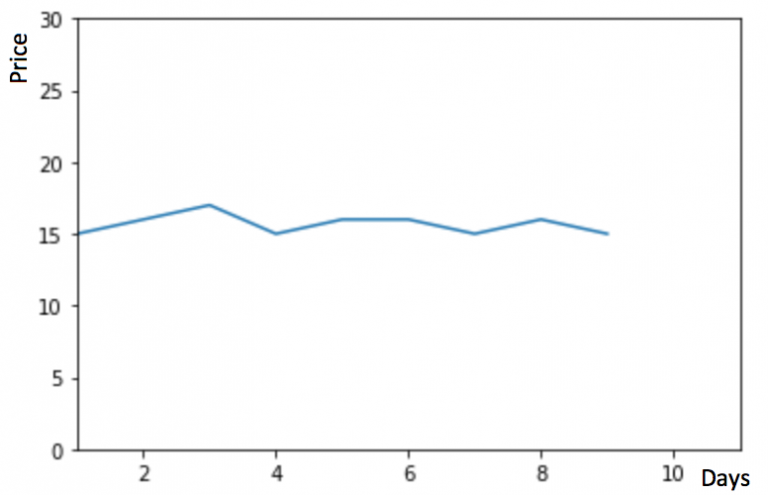
\includegraphics{image.png}
\caption{}
\end{figure}

We can infer from the graph that the price of the coin is stable from
the start. Many a times we are provided with a dataset, which is stable
throughout it's time period. If we want to forecast the price for the
next day, we can simply take the last day value and estimate the same
value for the next day. Such forecasting technique which assumes that
the next expected point is equal to the last observed point is called
Naive Method.

\begin{figure}
\centering
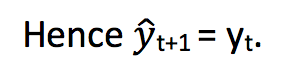
\includegraphics{image1.png}
\caption{}
\end{figure}

Now we will implement the Naive method to forecast the prices for test
data.

    \begin{Verbatim}[commandchars=\\\{\}]
{\color{incolor}In [{\color{incolor}197}]:} \PY{c+c1}{\PYZsh{}\PYZsh{}\PYZsh{}\PYZsh{} TODO}
          \PY{n}{dd}\PY{o}{=} \PY{n}{np}\PY{o}{.}\PY{n}{asarray}\PY{p}{(}\PY{n}{train}\PY{p}{[}\PY{l+s+s1}{\PYZsq{}}\PY{l+s+s1}{Bookings}\PY{l+s+s1}{\PYZsq{}}\PY{p}{]}\PY{o}{.}\PY{n}{count}\PY{p}{)}
          \PY{n}{y\PYZus{}hat} \PY{o}{=} \PY{n}{test}\PY{o}{.}\PY{n}{copy}\PY{p}{(}\PY{p}{)}
          \PY{n}{y\PYZus{}hat}\PY{p}{[}\PY{l+s+s1}{\PYZsq{}}\PY{l+s+s1}{naive}\PY{l+s+s1}{\PYZsq{}}\PY{p}{]} \PY{o}{=} \PY{n}{dd}\PY{p}{[}\PY{n+nb}{len}\PY{p}{(}\PY{n}{dd}\PY{p}{)}\PY{o}{\PYZhy{}}\PY{l+m+mi}{1}\PY{p}{]}
          
          
          
          \PY{n}{plt}\PY{o}{.}\PY{n}{figure}\PY{p}{(}\PY{n}{figsize}\PY{o}{=}\PY{p}{(}\PY{l+m+mi}{12}\PY{p}{,}\PY{l+m+mi}{8}\PY{p}{)}\PY{p}{)}
          \PY{n}{plt}\PY{o}{.}\PY{n}{plot}\PY{p}{(}\PY{n}{train}\PY{o}{.}\PY{n}{index}\PY{p}{,} \PY{n}{train}\PY{p}{[}\PY{l+s+s1}{\PYZsq{}}\PY{l+s+s1}{Count}\PY{l+s+s1}{\PYZsq{}}\PY{p}{]}\PY{p}{,} \PY{n}{label}\PY{o}{=}\PY{l+s+s1}{\PYZsq{}}\PY{l+s+s1}{Train}\PY{l+s+s1}{\PYZsq{}}\PY{p}{)}
          \PY{n}{plt}\PY{o}{.}\PY{n}{plot}\PY{p}{(}\PY{n}{test}\PY{o}{.}\PY{n}{index}\PY{p}{,}\PY{n}{test}\PY{p}{[}\PY{l+s+s1}{\PYZsq{}}\PY{l+s+s1}{Count}\PY{l+s+s1}{\PYZsq{}}\PY{p}{]}\PY{p}{,} \PY{n}{label}\PY{o}{=}\PY{l+s+s1}{\PYZsq{}}\PY{l+s+s1}{Test}\PY{l+s+s1}{\PYZsq{}}\PY{p}{)}
          \PY{n}{plt}\PY{o}{.}\PY{n}{plot}\PY{p}{(}\PY{n}{y\PYZus{}hat}\PY{o}{.}\PY{n}{index}\PY{p}{,}\PY{n}{y\PYZus{}hat}\PY{p}{[}\PY{l+s+s1}{\PYZsq{}}\PY{l+s+s1}{naive}\PY{l+s+s1}{\PYZsq{}}\PY{p}{]}\PY{p}{,} \PY{n}{label}\PY{o}{=}\PY{l+s+s1}{\PYZsq{}}\PY{l+s+s1}{Naive Forecast}\PY{l+s+s1}{\PYZsq{}}\PY{p}{)}
          \PY{n}{plt}\PY{o}{.}\PY{n}{legend}\PY{p}{(}\PY{n}{loc}\PY{o}{=}\PY{l+s+s1}{\PYZsq{}}\PY{l+s+s1}{best}\PY{l+s+s1}{\PYZsq{}}\PY{p}{)}
          \PY{n}{plt}\PY{o}{.}\PY{n}{title}\PY{p}{(}\PY{l+s+s2}{\PYZdq{}}\PY{l+s+s2}{Naive Forecast}\PY{l+s+s2}{\PYZdq{}}\PY{p}{)}
          \PY{n}{plt}\PY{o}{.}\PY{n}{show}\PY{p}{(}\PY{p}{)}
\end{Verbatim}


    \begin{Verbatim}[commandchars=\\\{\}]

        ---------------------------------------------------------------------------

        IndexError                                Traceback (most recent call last)

        <ipython-input-197-ece64aa3d409> in <module>()
          1 \#\#\#\# TODO
          2 dd= np.asarray(train['Bookings'].count)
    ----> 3 print(dd[-1])
          4 y\_hat = test.copy()
          5 y\_hat['naive'] = dd[-1]


        IndexError: too many indices for array

    \end{Verbatim}

    \subsection{Method 2: -- Simple Average}\label{method-2-simple-average}

Consider the graph given below. Let's assume that the y-axis depicts the
price of a coin and x-axis depicts the time(days).

We can infer from the graph that the price of the coin is increasing and
decreasing randomly by a small margin, such that the average remains
constant. Many a times we are provided with a dataset, which though
varies by a small margin throughout it's time period, but the average at
each time period remains constant. In such a case we can forecast the
price of the next day somewhere similar to the average of all the past
days.

Such forecasting technique which forecasts the expected value equal to
the average of all previously observed points is called Simple Average
technique.

We take all the values previously known, calculate the average and take
it as the next value. Of course it won't be it exact, but somewhat
close. As a forecasting method, there are actually situations where this
technique works the best.

    \begin{Verbatim}[commandchars=\\\{\}]
{\color{incolor}In [{\color{incolor}78}]:} \PY{n}{y\PYZus{}hat\PYZus{}avg} \PY{o}{=} \PY{n}{test}\PY{o}{.}\PY{n}{copy}\PY{p}{(}\PY{p}{)}
         \PY{n}{y\PYZus{}hat\PYZus{}avg}\PY{p}{[}\PY{l+s+s1}{\PYZsq{}}\PY{l+s+s1}{avg\PYZus{}forecast}\PY{l+s+s1}{\PYZsq{}}\PY{p}{]} \PY{o}{=} \PY{n}{train}\PY{p}{[}\PY{l+s+s1}{\PYZsq{}}\PY{l+s+s1}{Bookings}\PY{l+s+s1}{\PYZsq{}}\PY{p}{]}\PY{o}{.}\PY{n}{mean}\PY{p}{(}\PY{p}{)}
         \PY{n}{plt}\PY{o}{.}\PY{n}{figure}\PY{p}{(}\PY{n}{figsize}\PY{o}{=}\PY{p}{(}\PY{l+m+mi}{12}\PY{p}{,}\PY{l+m+mi}{8}\PY{p}{)}\PY{p}{)}
         \PY{n}{plt}\PY{o}{.}\PY{n}{plot}\PY{p}{(}\PY{n}{train}\PY{o}{.}\PY{n}{index}\PY{p}{,} \PY{n}{train}\PY{p}{[}\PY{l+s+s1}{\PYZsq{}}\PY{l+s+s1}{Bookings}\PY{l+s+s1}{\PYZsq{}}\PY{p}{]}\PY{p}{,} \PY{n}{label}\PY{o}{=}\PY{l+s+s1}{\PYZsq{}}\PY{l+s+s1}{Train}\PY{l+s+s1}{\PYZsq{}}\PY{p}{)}
         \PY{n}{plt}\PY{o}{.}\PY{n}{plot}\PY{p}{(}\PY{n}{test}\PY{o}{.}\PY{n}{index}\PY{p}{,}\PY{n}{test}\PY{p}{[}\PY{l+s+s1}{\PYZsq{}}\PY{l+s+s1}{Bookings}\PY{l+s+s1}{\PYZsq{}}\PY{p}{]}\PY{p}{,} \PY{n}{label}\PY{o}{=}\PY{l+s+s1}{\PYZsq{}}\PY{l+s+s1}{Test}\PY{l+s+s1}{\PYZsq{}}\PY{p}{)}
         \PY{n}{plt}\PY{o}{.}\PY{n}{plot}\PY{p}{(}\PY{n}{y\PYZus{}hat\PYZus{}avg}\PY{p}{[}\PY{l+s+s1}{\PYZsq{}}\PY{l+s+s1}{avg\PYZus{}forecast}\PY{l+s+s1}{\PYZsq{}}\PY{p}{]}\PY{p}{,} \PY{n}{label}\PY{o}{=}\PY{l+s+s1}{\PYZsq{}}\PY{l+s+s1}{Average Forecast}\PY{l+s+s1}{\PYZsq{}}\PY{p}{)}
         \PY{n}{plt}\PY{o}{.}\PY{n}{legend}\PY{p}{(}\PY{n}{loc}\PY{o}{=}\PY{l+s+s1}{\PYZsq{}}\PY{l+s+s1}{best}\PY{l+s+s1}{\PYZsq{}}\PY{p}{)}
         \PY{n}{plt}\PY{o}{.}\PY{n}{show}\PY{p}{(}\PY{p}{)}
\end{Verbatim}


    \begin{center}
    \adjustimage{max size={0.9\linewidth}{0.9\paperheight}}{output_11_0.png}
    \end{center}
    { \hspace*{\fill} \\}
    
    \begin{Verbatim}[commandchars=\\\{\}]
{\color{incolor}In [{\color{incolor} }]:} \PY{n}{We} \PY{n}{will} \PY{n}{now} \PY{n}{calculate} \PY{n}{RMSE} \PY{n}{to} \PY{n}{check} \PY{n}{to} \PY{n}{accuracy} \PY{n}{of} \PY{n}{our} \PY{n}{model}\PY{o}{.}
\end{Verbatim}


    \begin{Verbatim}[commandchars=\\\{\}]
{\color{incolor}In [{\color{incolor}84}]:} \PY{n}{rms} \PY{o}{=} \PY{n}{sqrt}\PY{p}{(}\PY{n}{mean\PYZus{}squared\PYZus{}error}\PY{p}{(}\PY{n}{test}\PY{p}{[}\PY{l+s+s1}{\PYZsq{}}\PY{l+s+s1}{Bookings}\PY{l+s+s1}{\PYZsq{}}\PY{p}{]}\PY{p}{,} \PY{n}{y\PYZus{}hat\PYZus{}avg}\PY{o}{.}\PY{n}{avg\PYZus{}forecast}\PY{p}{)}\PY{p}{)}
         \PY{n+nb}{print}\PY{p}{(}\PY{n}{rms}\PY{p}{)}
\end{Verbatim}


    \begin{Verbatim}[commandchars=\\\{\}]
8315.512361444322

    \end{Verbatim}

    We can see that this model didn't improve our score. Hence we can infer
from the score that this method works best when the average at each time
period remains constant. Though the score of Naive method is better than
Average method, but this does not mean that the Naive method is better
than Average method on all datasets. We should move step by step to each
model and confirm whether it improves our model or not.

    \subsection{Method 3 -- Moving Average}\label{method-3-moving-average}

Consider the graph given below. Let's assume that the y-axis depicts the
price of a coin and x-axis depicts the time(days).

\begin{figure}
\centering
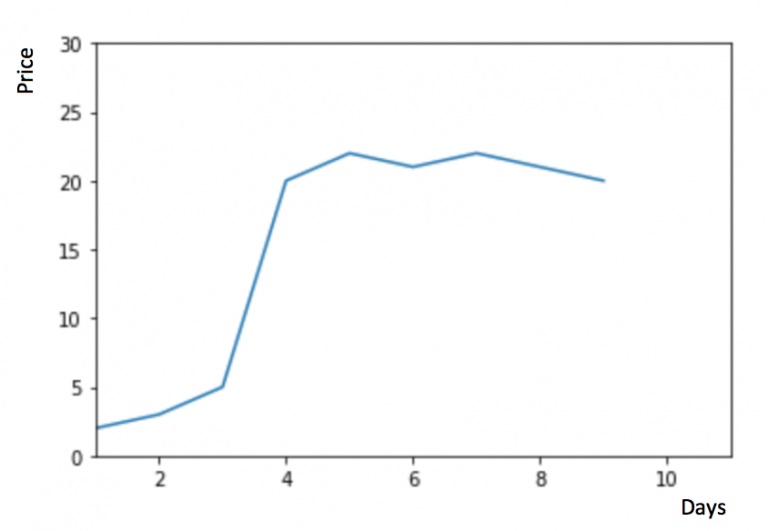
\includegraphics{image5.png}
\caption{}
\end{figure}

We can infer from the graph that the prices of the coin increased some
time periods ago by a big margin but now they are stable. Many a times
we are provided with a dataset, in which the prices/sales of the object
increased/decreased sharply some time periods ago. In order to use the
previous Average method, we have to use the mean of all the previous
data, but using all the previous data doesn't sound right.

Using the prices of the initial period would highly affect the forecast
for the next period. Therefore as an improvement over simple average, we
will take the average of the prices for last few time periods only.
Obviously the thinking here is that only the recent values matter. Such
forecasting technique which uses window of time period for calculating
the average is called Moving Average technique. Calculation of the
moving average involves what is sometimes called a ``sliding window'' of
size n.

Using a simple moving average model, we forecast the next value(s) in a
time series based on the average of a fixed finite number `p' of the
previous values. Thus, for all i \textgreater{} p

\begin{figure}
\centering
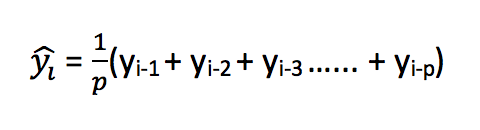
\includegraphics{image6.png}
\caption{}
\end{figure}

A moving average can actually be quite effective, especially if you pick
the right p for the series.

    \begin{Verbatim}[commandchars=\\\{\}]
{\color{incolor}In [{\color{incolor}89}]:} \PY{n}{y\PYZus{}hat\PYZus{}avg} \PY{o}{=} \PY{n}{test}\PY{o}{.}\PY{n}{copy}\PY{p}{(}\PY{p}{)}
         \PY{n}{y\PYZus{}hat\PYZus{}avg}\PY{p}{[}\PY{l+s+s1}{\PYZsq{}}\PY{l+s+s1}{moving\PYZus{}avg\PYZus{}forecast}\PY{l+s+s1}{\PYZsq{}}\PY{p}{]} \PY{o}{=} \PY{n}{train}\PY{p}{[}\PY{l+s+s1}{\PYZsq{}}\PY{l+s+s1}{Bookings}\PY{l+s+s1}{\PYZsq{}}\PY{p}{]}\PY{o}{.}\PY{n}{rolling}\PY{p}{(}\PY{l+m+mi}{2}\PY{p}{)}\PY{o}{.}\PY{n}{mean}\PY{p}{(}\PY{p}{)}\PY{o}{.}\PY{n}{iloc}\PY{p}{[}\PY{o}{\PYZhy{}}\PY{l+m+mi}{1}\PY{p}{]}
         \PY{n}{plt}\PY{o}{.}\PY{n}{figure}\PY{p}{(}\PY{n}{figsize}\PY{o}{=}\PY{p}{(}\PY{l+m+mi}{16}\PY{p}{,}\PY{l+m+mi}{8}\PY{p}{)}\PY{p}{)}
         \PY{n}{plt}\PY{o}{.}\PY{n}{plot}\PY{p}{(}\PY{n}{train}\PY{o}{.}\PY{n}{index}\PY{p}{,} \PY{n}{train}\PY{p}{[}\PY{l+s+s1}{\PYZsq{}}\PY{l+s+s1}{Bookings}\PY{l+s+s1}{\PYZsq{}}\PY{p}{]}\PY{p}{,} \PY{n}{label}\PY{o}{=}\PY{l+s+s1}{\PYZsq{}}\PY{l+s+s1}{Train}\PY{l+s+s1}{\PYZsq{}}\PY{p}{)}
         \PY{n}{plt}\PY{o}{.}\PY{n}{plot}\PY{p}{(}\PY{n}{test}\PY{o}{.}\PY{n}{index}\PY{p}{,}\PY{n}{test}\PY{p}{[}\PY{l+s+s1}{\PYZsq{}}\PY{l+s+s1}{Bookings}\PY{l+s+s1}{\PYZsq{}}\PY{p}{]}\PY{p}{,} \PY{n}{label}\PY{o}{=}\PY{l+s+s1}{\PYZsq{}}\PY{l+s+s1}{Test}\PY{l+s+s1}{\PYZsq{}}\PY{p}{)}
         \PY{n}{plt}\PY{o}{.}\PY{n}{plot}\PY{p}{(}\PY{n}{y\PYZus{}hat\PYZus{}avg}\PY{p}{[}\PY{l+s+s1}{\PYZsq{}}\PY{l+s+s1}{moving\PYZus{}avg\PYZus{}forecast}\PY{l+s+s1}{\PYZsq{}}\PY{p}{]}\PY{p}{,} \PY{n}{label}\PY{o}{=}\PY{l+s+s1}{\PYZsq{}}\PY{l+s+s1}{Moving Average Forecast}\PY{l+s+s1}{\PYZsq{}}\PY{p}{)}
         \PY{n}{plt}\PY{o}{.}\PY{n}{legend}\PY{p}{(}\PY{n}{loc}\PY{o}{=}\PY{l+s+s1}{\PYZsq{}}\PY{l+s+s1}{best}\PY{l+s+s1}{\PYZsq{}}\PY{p}{)}
         \PY{n}{plt}\PY{o}{.}\PY{n}{show}\PY{p}{(}\PY{p}{)}
\end{Verbatim}


    \begin{center}
    \adjustimage{max size={0.9\linewidth}{0.9\paperheight}}{output_16_0.png}
    \end{center}
    { \hspace*{\fill} \\}
    
    We chose the data of last 2 months only. We will now calculate RMSE to
check to accuracy of our model.

    \begin{Verbatim}[commandchars=\\\{\}]
{\color{incolor}In [{\color{incolor}91}]:} \PY{n}{rms} \PY{o}{=} \PY{n}{sqrt}\PY{p}{(}\PY{n}{mean\PYZus{}squared\PYZus{}error}\PY{p}{(}\PY{n}{test}\PY{p}{[}\PY{l+s+s1}{\PYZsq{}}\PY{l+s+s1}{Bookings}\PY{l+s+s1}{\PYZsq{}}\PY{p}{]}\PY{p}{,} \PY{n}{y\PYZus{}hat\PYZus{}avg}\PY{o}{.}\PY{n}{moving\PYZus{}avg\PYZus{}forecast}\PY{p}{)}\PY{p}{)}
         \PY{n+nb}{print}\PY{p}{(}\PY{n}{rms}\PY{p}{)}
\end{Verbatim}


    \begin{Verbatim}[commandchars=\\\{\}]
3676.667864158161

    \end{Verbatim}

    We can see that Naive method outperforms both Average method and Moving
Average method for this dataset. Now we will look at Simple Exponential
Smoothing method and see how it performs.

An advancement over Moving average method is Weighted moving average
method. In the Moving average method as seen above, we equally weigh the
past `n' observations. But we might encounter situations where each of
the observation from the past `n' impacts the forecast in a different
way. Such a technique which weighs the past observations differently is
called Weighted Moving Average technique.

A weighted moving average is a moving average where within the sliding
window values are given different weights, typically so that more recent
points matter more. Ins

\begin{figure}
\centering
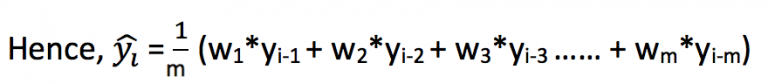
\includegraphics{image7.png}
\caption{}
\end{figure}

tead of selecting a window size, it requires a list of weights (which
should add up to 1). For example if we pick {[}0.40, 0.25, 0.20, 0.15{]}
as weights, we would be giving 40\%, 25\%, 20\% and 15\% to the last 4
points respectively.

    \subsection{Method 4 -- Simple Exponential
Smoothing}\label{method-4-simple-exponential-smoothing}

After we have understood the above methods, we can note that both Simple
average and Weighted moving average lie on completely opposite ends. We
would need something between these two extremes approaches which takes
into account all the data while weighing the data points differently.
For example it may be sensible to attach larger weights to more recent
observations than to observations from the distant past. The technique
which works on this principle is called Simple exponential smoothing.
Forecasts are calculated using weighted averages where the weights
decrease exponentially as observations come from further in the past,
the smallest weights are associated with the oldest observations:

\begin{figure}
\centering
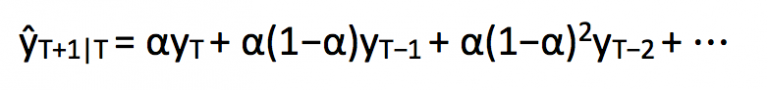
\includegraphics{image8.png}
\caption{}
\end{figure}

where 0≤ α ≤1 is the smoothing parameter.

The one-step-ahead forecast for time T+1 is a weighted average of all
the observations in the series y1,\ldots{},yT. The rate at which the
weights decrease is controlled by the parameter α.

If you stare at it just long enough, you will see that the expected
value ŷx is the sum of two products: α⋅yt and (1−α)⋅ŷ t-1.

Hence, it can also be written as :

\begin{figure}
\centering
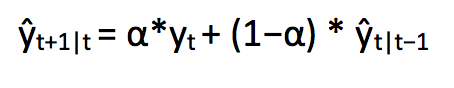
\includegraphics{image9.png}
\caption{}
\end{figure}

So essentially we've got a weighted moving average with two weights: α
and 1−α.

As we can see, 1−α is multiplied by the previous expected value ŷ x−1
which makes the expression recursive. And this is why this method is
called Exponential. The forecast at time t+1 is equal to a weighted
average between the most recent observation yt and the most recent
forecast ŷ t\textbar{}t−1.

    \begin{Verbatim}[commandchars=\\\{\}]
{\color{incolor}In [{\color{incolor}94}]:} \PY{k+kn}{from} \PY{n+nn}{statsmodels}\PY{n+nn}{.}\PY{n+nn}{tsa}\PY{n+nn}{.}\PY{n+nn}{api} \PY{k}{import} \PY{n}{ExponentialSmoothing}\PY{p}{,} \PY{n}{SimpleExpSmoothing}\PY{p}{,} \PY{n}{Holt}
         \PY{n}{y\PYZus{}hat\PYZus{}avg} \PY{o}{=} \PY{n}{test}\PY{o}{.}\PY{n}{copy}\PY{p}{(}\PY{p}{)}
         \PY{n}{fit2} \PY{o}{=} \PY{n}{SimpleExpSmoothing}\PY{p}{(}\PY{n}{np}\PY{o}{.}\PY{n}{asarray}\PY{p}{(}\PY{n}{train}\PY{p}{[}\PY{l+s+s1}{\PYZsq{}}\PY{l+s+s1}{Bookings}\PY{l+s+s1}{\PYZsq{}}\PY{p}{]}\PY{p}{)}\PY{p}{)}\PY{o}{.}\PY{n}{fit}\PY{p}{(}\PY{n}{smoothing\PYZus{}level}\PY{o}{=}\PY{l+m+mf}{0.9}\PY{p}{,}\PY{n}{optimized}\PY{o}{=}\PY{k+kc}{False}\PY{p}{)}
         \PY{n}{y\PYZus{}hat\PYZus{}avg}\PY{p}{[}\PY{l+s+s1}{\PYZsq{}}\PY{l+s+s1}{SES}\PY{l+s+s1}{\PYZsq{}}\PY{p}{]} \PY{o}{=} \PY{n}{fit2}\PY{o}{.}\PY{n}{forecast}\PY{p}{(}\PY{n+nb}{len}\PY{p}{(}\PY{n}{test}\PY{p}{)}\PY{p}{)}
         \PY{n}{plt}\PY{o}{.}\PY{n}{figure}\PY{p}{(}\PY{n}{figsize}\PY{o}{=}\PY{p}{(}\PY{l+m+mi}{16}\PY{p}{,}\PY{l+m+mi}{8}\PY{p}{)}\PY{p}{)}
         \PY{n}{plt}\PY{o}{.}\PY{n}{plot}\PY{p}{(}\PY{n}{train}\PY{o}{.}\PY{n}{index}\PY{p}{,} \PY{n}{train}\PY{p}{[}\PY{l+s+s1}{\PYZsq{}}\PY{l+s+s1}{Bookings}\PY{l+s+s1}{\PYZsq{}}\PY{p}{]}\PY{p}{,} \PY{n}{label}\PY{o}{=}\PY{l+s+s1}{\PYZsq{}}\PY{l+s+s1}{Train}\PY{l+s+s1}{\PYZsq{}}\PY{p}{)}
         \PY{n}{plt}\PY{o}{.}\PY{n}{plot}\PY{p}{(}\PY{n}{test}\PY{o}{.}\PY{n}{index}\PY{p}{,}\PY{n}{test}\PY{p}{[}\PY{l+s+s1}{\PYZsq{}}\PY{l+s+s1}{Bookings}\PY{l+s+s1}{\PYZsq{}}\PY{p}{]}\PY{p}{,} \PY{n}{label}\PY{o}{=}\PY{l+s+s1}{\PYZsq{}}\PY{l+s+s1}{Test}\PY{l+s+s1}{\PYZsq{}}\PY{p}{)}
         \PY{n}{plt}\PY{o}{.}\PY{n}{plot}\PY{p}{(}\PY{n}{y\PYZus{}hat\PYZus{}avg}\PY{p}{[}\PY{l+s+s1}{\PYZsq{}}\PY{l+s+s1}{SES}\PY{l+s+s1}{\PYZsq{}}\PY{p}{]}\PY{p}{,} \PY{n}{label}\PY{o}{=}\PY{l+s+s1}{\PYZsq{}}\PY{l+s+s1}{SES}\PY{l+s+s1}{\PYZsq{}}\PY{p}{)}
         \PY{n}{plt}\PY{o}{.}\PY{n}{legend}\PY{p}{(}\PY{n}{loc}\PY{o}{=}\PY{l+s+s1}{\PYZsq{}}\PY{l+s+s1}{best}\PY{l+s+s1}{\PYZsq{}}\PY{p}{)}
         \PY{n}{plt}\PY{o}{.}\PY{n}{show}\PY{p}{(}\PY{p}{)}
\end{Verbatim}


    \begin{center}
    \adjustimage{max size={0.9\linewidth}{0.9\paperheight}}{output_21_0.png}
    \end{center}
    { \hspace*{\fill} \\}
    
    We will now calculate RMSE to check to accuracy of our model.

    \begin{Verbatim}[commandchars=\\\{\}]
{\color{incolor}In [{\color{incolor}96}]:} \PY{n}{rms} \PY{o}{=} \PY{n}{sqrt}\PY{p}{(}\PY{n}{mean\PYZus{}squared\PYZus{}error}\PY{p}{(}\PY{n}{test}\PY{p}{[}\PY{l+s+s1}{\PYZsq{}}\PY{l+s+s1}{Bookings}\PY{l+s+s1}{\PYZsq{}}\PY{p}{]}\PY{p}{,} \PY{n}{y\PYZus{}hat\PYZus{}avg}\PY{o}{.}\PY{n}{SES}\PY{p}{)}\PY{p}{)}
         \PY{n+nb}{print}\PY{p}{(}\PY{n}{rms}\PY{p}{)}
\end{Verbatim}


    \begin{Verbatim}[commandchars=\\\{\}]
2911.005572337132

    \end{Verbatim}

    \subsection{Method 5 -- Holt's Linear Trend
method}\label{method-5-holts-linear-trend-method}

We have now learnt several methods to forecast but we can see that these
models don't work well on data with high variations. Consider that the
price of the bitcoin is increasing.

\begin{figure}
\centering
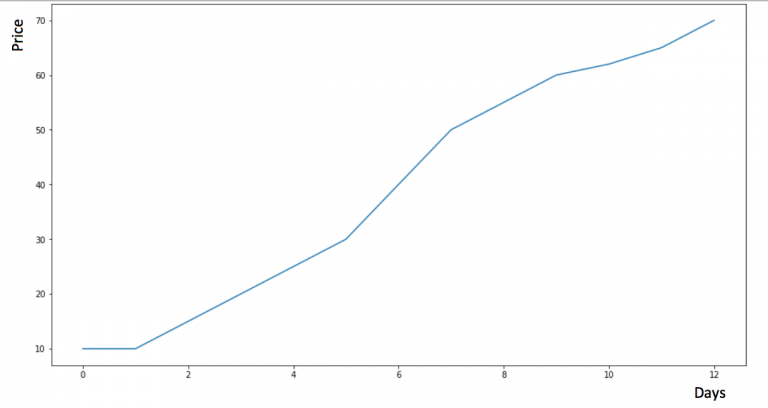
\includegraphics{image10.png}
\caption{}
\end{figure}

If we use any of the above methods, it won't take into account this
trend. Trend is the general pattern of prices that we observe over a
period of time. In this case we can see that there is an increasing
trend.

Although each one of these methods can be applied to the trend as well.
E.g. the Naive method would assume that trend between last two points is
going to stay the same, or we could average all slopes between all
points to get an average trend, use a moving trend average or apply
exponential smoothing.

But we need a method that can map the trend accurately without any
assumptions. Such a method that takes into account the trend of the
dataset is called Holt's Linear Trend method.

Each Time series dataset can be decomposed into it's componenets which
are Trend, Seasonality and Residual. Any dataset that follows a trend
can use Holt's linear trend method for forecasting.

    \begin{Verbatim}[commandchars=\\\{\}]
{\color{incolor}In [{\color{incolor}103}]:} \PY{k+kn}{import} \PY{n+nn}{statsmodels}\PY{n+nn}{.}\PY{n+nn}{api} \PY{k}{as} \PY{n+nn}{sm}
          
          \PY{n}{sm}\PY{o}{.}\PY{n}{tsa}\PY{o}{.}\PY{n}{seasonal\PYZus{}decompose}\PY{p}{(}\PY{n}{train}\PY{p}{[}\PY{l+s+s1}{\PYZsq{}}\PY{l+s+s1}{Bookings}\PY{l+s+s1}{\PYZsq{}}\PY{p}{]}\PY{p}{)}\PY{o}{.}\PY{n}{plot}\PY{p}{(}\PY{p}{)}
          
          \PY{n}{result} \PY{o}{=} \PY{n}{sm}\PY{o}{.}\PY{n}{tsa}\PY{o}{.}\PY{n}{stattools}\PY{o}{.}\PY{n}{adfuller}\PY{p}{(}\PY{n}{train}\PY{p}{[}\PY{l+s+s1}{\PYZsq{}}\PY{l+s+s1}{Bookings}\PY{l+s+s1}{\PYZsq{}}\PY{p}{]}\PY{p}{)}
          \PY{n}{plt}\PY{o}{.}\PY{n}{title}\PY{p}{(}\PY{l+s+s1}{\PYZsq{}}\PY{l+s+s1}{Decomposition plot}\PY{l+s+s1}{\PYZsq{}}\PY{p}{)}
          \PY{n}{plt}\PY{o}{.}\PY{n}{show}\PY{p}{(}\PY{p}{)}
\end{Verbatim}


    \begin{center}
    \adjustimage{max size={0.9\linewidth}{0.9\paperheight}}{output_25_0.png}
    \end{center}
    { \hspace*{\fill} \\}
    
    We can see from the graphs obtained that this dataset follows an
increasing trend. Hence we can use Holt's linear trend to forecast the
future prices.

Holt extended simple exponential smoothing to allow forecasting of data
with a trend. It is nothing more than exponential smoothing applied to
both level(the average value in the series) and trend. To express this
in mathematical notation we now need three equations: one for level, one
for the trend and one to combine the level and trend to get the expected
forecast ŷ

\begin{figure}
\centering
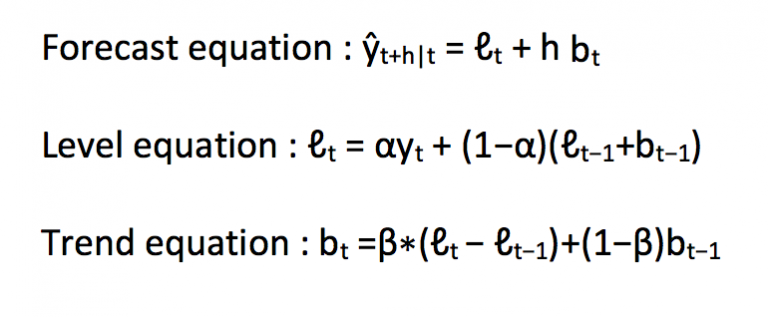
\includegraphics{image11.png}
\caption{}
\end{figure}

The values we predicted in the above algorithms are called Level. In the
above three equations, you can notice that we have added level and trend
to generate the forecast equation.

As with simple exponential smoothing, the level equation here shows that
it is a weighted average of observation and the within-sample
one-step-ahead forecast The trend equation shows that it is a weighted
average of the estimated trend at time t based on ℓ(t)−ℓ(t−1) and
b(t−1), the previous estimate of the trend.

We will add these equations to generate Forecast equation. We can also
generate a multiplicative forecast equation by multiplying trend and
level instead of adding it. When the trend increases or decreases
linearly, additive equation is used whereas when the trend increases of
decreases exponentially, multiplicative equation is used.Practice shows
that multiplicative is a more stable predictor, the additive method
however is simpler to understand.

\begin{figure}
\centering
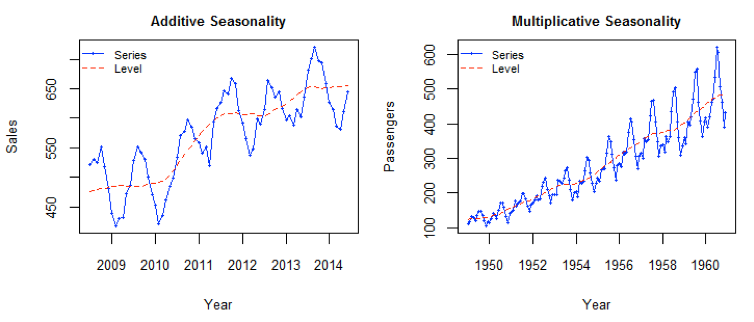
\includegraphics{image12.png}
\caption{}
\end{figure}

    \begin{Verbatim}[commandchars=\\\{\}]
{\color{incolor}In [{\color{incolor}137}]:} \PY{n}{y\PYZus{}hat\PYZus{}avg} \PY{o}{=} \PY{n}{test}\PY{o}{.}\PY{n}{copy}\PY{p}{(}\PY{p}{)}
          
          \PY{n}{fit1} \PY{o}{=} \PY{n}{Holt}\PY{p}{(}\PY{n}{np}\PY{o}{.}\PY{n}{asarray}\PY{p}{(}\PY{n}{train}\PY{p}{[}\PY{l+s+s1}{\PYZsq{}}\PY{l+s+s1}{Bookings}\PY{l+s+s1}{\PYZsq{}}\PY{p}{]}\PY{p}{)}\PY{p}{)}\PY{o}{.}\PY{n}{fit}\PY{p}{(}\PY{n}{smoothing\PYZus{}level} \PY{o}{=} \PY{l+m+mf}{0.5}\PY{p}{,}\PY{n}{smoothing\PYZus{}slope} \PY{o}{=} \PY{l+m+mf}{0.1}\PY{p}{)}
          \PY{n}{y\PYZus{}hat\PYZus{}avg}\PY{p}{[}\PY{l+s+s1}{\PYZsq{}}\PY{l+s+s1}{Holt\PYZus{}linear}\PY{l+s+s1}{\PYZsq{}}\PY{p}{]} \PY{o}{=} \PY{n}{fit1}\PY{o}{.}\PY{n}{forecast}\PY{p}{(}\PY{n+nb}{len}\PY{p}{(}\PY{n}{test}\PY{p}{)}\PY{p}{)}
          
          \PY{n}{plt}\PY{o}{.}\PY{n}{figure}\PY{p}{(}\PY{n}{figsize}\PY{o}{=}\PY{p}{(}\PY{l+m+mi}{16}\PY{p}{,}\PY{l+m+mi}{8}\PY{p}{)}\PY{p}{)}
          \PY{n}{plt}\PY{o}{.}\PY{n}{plot}\PY{p}{(}\PY{n}{train}\PY{o}{.}\PY{n}{index}\PY{p}{,} \PY{n}{train}\PY{p}{[}\PY{l+s+s1}{\PYZsq{}}\PY{l+s+s1}{Bookings}\PY{l+s+s1}{\PYZsq{}}\PY{p}{]}\PY{p}{,} \PY{n}{label}\PY{o}{=}\PY{l+s+s1}{\PYZsq{}}\PY{l+s+s1}{Train}\PY{l+s+s1}{\PYZsq{}}\PY{p}{)}
          \PY{n}{plt}\PY{o}{.}\PY{n}{plot}\PY{p}{(}\PY{n}{test}\PY{o}{.}\PY{n}{index}\PY{p}{,}\PY{n}{test}\PY{p}{[}\PY{l+s+s1}{\PYZsq{}}\PY{l+s+s1}{Bookings}\PY{l+s+s1}{\PYZsq{}}\PY{p}{]}\PY{p}{,} \PY{n}{label}\PY{o}{=}\PY{l+s+s1}{\PYZsq{}}\PY{l+s+s1}{Test}\PY{l+s+s1}{\PYZsq{}}\PY{p}{)}
          \PY{n}{plt}\PY{o}{.}\PY{n}{plot}\PY{p}{(}\PY{n}{y\PYZus{}hat\PYZus{}avg}\PY{p}{[}\PY{l+s+s1}{\PYZsq{}}\PY{l+s+s1}{Holt\PYZus{}linear}\PY{l+s+s1}{\PYZsq{}}\PY{p}{]}\PY{p}{,} \PY{n}{label}\PY{o}{=}\PY{l+s+s1}{\PYZsq{}}\PY{l+s+s1}{Holt\PYZus{}linear}\PY{l+s+s1}{\PYZsq{}}\PY{p}{)}
          \PY{n}{plt}\PY{o}{.}\PY{n}{legend}\PY{p}{(}\PY{n}{loc}\PY{o}{=}\PY{l+s+s1}{\PYZsq{}}\PY{l+s+s1}{best}\PY{l+s+s1}{\PYZsq{}}\PY{p}{)}
          \PY{n}{plt}\PY{o}{.}\PY{n}{show}\PY{p}{(}\PY{p}{)}
\end{Verbatim}


    \begin{center}
    \adjustimage{max size={0.9\linewidth}{0.9\paperheight}}{output_27_0.png}
    \end{center}
    { \hspace*{\fill} \\}
    
    We will now calculate RMSE to check to accuracy of our model.

    \begin{Verbatim}[commandchars=\\\{\}]
{\color{incolor}In [{\color{incolor}138}]:} \PY{n}{rms} \PY{o}{=} \PY{n}{sqrt}\PY{p}{(}\PY{n}{mean\PYZus{}squared\PYZus{}error}\PY{p}{(}\PY{n}{test}\PY{p}{[}\PY{l+s+s1}{\PYZsq{}}\PY{l+s+s1}{Bookings}\PY{l+s+s1}{\PYZsq{}}\PY{p}{]}\PY{p}{,} \PY{n}{y\PYZus{}hat\PYZus{}avg}\PY{o}{.}\PY{n}{Holt\PYZus{}linear}\PY{p}{)}\PY{p}{)}
          \PY{n+nb}{print}\PY{p}{(}\PY{n}{rms}\PY{p}{)}
\end{Verbatim}


    \begin{Verbatim}[commandchars=\\\{\}]
2681.032229524646

    \end{Verbatim}

    We can see that this method maps the trend accurately and hence provides
a better solution when compared with above models. We can still tune the
parameters to get even a better model.

    \subsection{Method 6 -- Holt-Winters
Method}\label{method-6-holt-winters-method}

So let's introduce a new term which will be used in this algorithm.
Consider a hotel located on a hill station. It experiences high visits
during the summer season whereas the visitors during the rest of the
year are comparatively very less. Hence the profit earned by the owner
will be far better in summer season than in any other season. This
pattern will repeat itself every year. Such a repetition is called
Seasonality. Datasets which show a similar set of pattern after fixed
intervals of a time period suffer from seasonality.

\begin{figure}
\centering
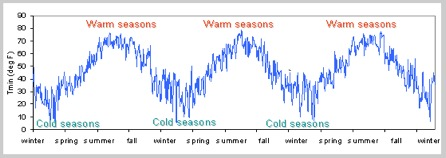
\includegraphics{image13.png}
\caption{}
\end{figure}

The above mentioned models don't take into account the seasonality of
the dataset while forecasting. Hence we need a method that takes into
account both trend and seasonality to forecast future prices. One such
algorithm that we can use in such a scenario is Holt's Winter method.
The idea behind triple exponential smoothing(Holt's Winter) is to apply
exponential smoothing to the seasonal components in addition to level
and trend.

Using Holt's winter method will be the best option among the rest of the
models beacuse of the seasonality factor. The Holt-Winters seasonal
method comprises the forecast equation and three smoothing equations ---
one for the level ℓt, one for trend bt and one for the seasonal
component denoted by st, with smoothing parameters α, β and γ.

\begin{figure}
\centering
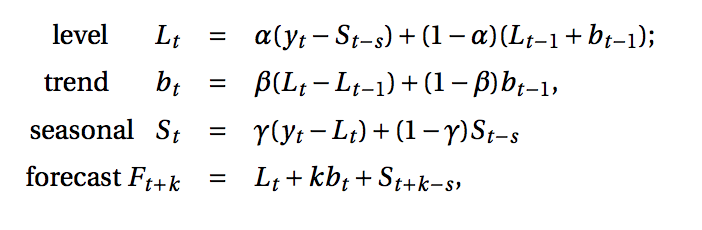
\includegraphics{image14.png}
\caption{}
\end{figure}

where s is the length of the seasonal cycle, for 0 ≤ α ≤ 1, 0 ≤ β ≤ 1
and 0 ≤ γ ≤ 1.

The level equation shows a weighted average between the seasonally
adjusted observation and the non-seasonal forecast for time t. The trend
equation is identical to Holt's linear method. The seasonal equation
shows a weighted average between the current seasonal index, and the
seasonal index of the same season last year (i.e., s time periods ago).

In this method also, we can implement both additive and multiplicative
technique. The additive method is preferred when the seasonal variations
are roughly constant through the series, while the multiplicative method
is preferred when the seasonal variations are changing proportional to
the level of the series.

    \begin{Verbatim}[commandchars=\\\{\}]
{\color{incolor}In [{\color{incolor}193}]:} \PY{n}{y\PYZus{}hat\PYZus{}avg} \PY{o}{=} \PY{n}{test}\PY{o}{.}\PY{n}{copy}\PY{p}{(}\PY{p}{)}
          \PY{n}{fit1} \PY{o}{=} \PY{n}{ExponentialSmoothing}\PY{p}{(}\PY{n}{np}\PY{o}{.}\PY{n}{asarray}\PY{p}{(}\PY{n}{train}\PY{p}{[}\PY{l+s+s1}{\PYZsq{}}\PY{l+s+s1}{Bookings}\PY{l+s+s1}{\PYZsq{}}\PY{p}{]}\PY{p}{)}\PY{p}{,}
                                      \PY{n}{seasonal\PYZus{}periods}\PY{o}{=}\PY{l+m+mi}{12}\PY{p}{,}
                                      \PY{n}{trend}\PY{o}{=}\PY{l+s+s1}{\PYZsq{}}\PY{l+s+s1}{add}\PY{l+s+s1}{\PYZsq{}}\PY{p}{,} 
                                      \PY{n}{seasonal}\PY{o}{=}\PY{l+s+s1}{\PYZsq{}}\PY{l+s+s1}{add}\PY{l+s+s1}{\PYZsq{}}\PY{p}{,}\PY{p}{)}\PY{o}{.}\PY{n}{fit}\PY{p}{(}\PY{n}{smoothing\PYZus{}level} \PY{o}{=} \PY{l+m+mf}{0.7}\PY{p}{,} \PY{n}{optimized}\PY{o}{=}\PY{k+kc}{True}\PY{p}{)}
          \PY{n}{y\PYZus{}hat\PYZus{}avg}\PY{p}{[}\PY{l+s+s1}{\PYZsq{}}\PY{l+s+s1}{Holt\PYZus{}Winter}\PY{l+s+s1}{\PYZsq{}}\PY{p}{]} \PY{o}{=} \PY{n}{fit1}\PY{o}{.}\PY{n}{forecast}\PY{p}{(}\PY{n+nb}{len}\PY{p}{(}\PY{n}{test}\PY{p}{)}\PY{p}{)}
          \PY{n}{plt}\PY{o}{.}\PY{n}{figure}\PY{p}{(}\PY{n}{figsize}\PY{o}{=}\PY{p}{(}\PY{l+m+mi}{16}\PY{p}{,}\PY{l+m+mi}{8}\PY{p}{)}\PY{p}{)}
          \PY{n}{plt}\PY{o}{.}\PY{n}{plot}\PY{p}{(}\PY{n}{train}\PY{o}{.}\PY{n}{index}\PY{p}{,} \PY{n}{train}\PY{p}{[}\PY{l+s+s1}{\PYZsq{}}\PY{l+s+s1}{Bookings}\PY{l+s+s1}{\PYZsq{}}\PY{p}{]}\PY{p}{,} \PY{n}{label}\PY{o}{=}\PY{l+s+s1}{\PYZsq{}}\PY{l+s+s1}{Train}\PY{l+s+s1}{\PYZsq{}}\PY{p}{)}
          \PY{n}{plt}\PY{o}{.}\PY{n}{plot}\PY{p}{(}\PY{n}{test}\PY{o}{.}\PY{n}{index}\PY{p}{,}\PY{n}{test}\PY{p}{[}\PY{l+s+s1}{\PYZsq{}}\PY{l+s+s1}{Bookings}\PY{l+s+s1}{\PYZsq{}}\PY{p}{]}\PY{p}{,} \PY{n}{label}\PY{o}{=}\PY{l+s+s1}{\PYZsq{}}\PY{l+s+s1}{Test}\PY{l+s+s1}{\PYZsq{}}\PY{p}{)}
          \PY{n}{plt}\PY{o}{.}\PY{n}{plot}\PY{p}{(}\PY{n}{y\PYZus{}hat\PYZus{}avg}\PY{p}{[}\PY{l+s+s1}{\PYZsq{}}\PY{l+s+s1}{Holt\PYZus{}Winter}\PY{l+s+s1}{\PYZsq{}}\PY{p}{]}\PY{p}{,} \PY{n}{label}\PY{o}{=}\PY{l+s+s1}{\PYZsq{}}\PY{l+s+s1}{Holt\PYZus{}Winter}\PY{l+s+s1}{\PYZsq{}}\PY{p}{)}
          \PY{n}{plt}\PY{o}{.}\PY{n}{legend}\PY{p}{(}\PY{n}{loc}\PY{o}{=}\PY{l+s+s1}{\PYZsq{}}\PY{l+s+s1}{best}\PY{l+s+s1}{\PYZsq{}}\PY{p}{)}
          \PY{n}{plt}\PY{o}{.}\PY{n}{grid}\PY{p}{(}\PY{l+s+s1}{\PYZsq{}}\PY{l+s+s1}{on}\PY{l+s+s1}{\PYZsq{}}\PY{p}{)}
          \PY{n}{plt}\PY{o}{.}\PY{n}{show}\PY{p}{(}\PY{p}{)}
\end{Verbatim}


    \begin{Verbatim}[commandchars=\\\{\}]
/home/emi/anaconda3/lib/python3.6/site-packages/matplotlib/cbook/deprecation.py:107: MatplotlibDeprecationWarning: Passing one of 'on', 'true', 'off', 'false' as a boolean is deprecated; use an actual boolean (True/False) instead.
  warnings.warn(message, mplDeprecation, stacklevel=1)

    \end{Verbatim}

    \begin{center}
    \adjustimage{max size={0.9\linewidth}{0.9\paperheight}}{output_32_1.png}
    \end{center}
    { \hspace*{\fill} \\}
    
    \begin{Verbatim}[commandchars=\\\{\}]
{\color{incolor}In [{\color{incolor}194}]:} \PY{n}{rms} \PY{o}{=} \PY{n}{sqrt}\PY{p}{(}\PY{n}{mean\PYZus{}squared\PYZus{}error}\PY{p}{(}\PY{n}{test}\PY{p}{[}\PY{l+s+s1}{\PYZsq{}}\PY{l+s+s1}{Bookings}\PY{l+s+s1}{\PYZsq{}}\PY{p}{]}\PY{p}{,} \PY{n}{y\PYZus{}hat\PYZus{}avg}\PY{o}{.}\PY{n}{Holt\PYZus{}Winter}\PY{p}{)}\PY{p}{)}
          \PY{n+nb}{print}\PY{p}{(}\PY{n}{rms}\PY{p}{)}
\end{Verbatim}


    \begin{Verbatim}[commandchars=\\\{\}]
1860.8735902750327

    \end{Verbatim}


    % Add a bibliography block to the postdoc
    
    
    
    \end{document}
